\section{Agent Swarm}
The primary challenge of existing agent-based systems lies in their reliance on {sequential execution} of reasoning and tool-calling steps. While this structure may be effective for simpler, short-horizon tasks, it becomes inadequate as the complexity of the task increases and the accumulated context grows. As tasks evolve to contain broad information gathering and intricate, multi-branch reasoning, sequential systems often encounter significant bottlenecks \citep{anthropicbuildmultiagent,opus45report,claudemultiagent}. The limited capacity of a single agent working through each step one by one can lead to the exhaustion of practical reasoning depth and tool-call budgets, ultimately hindering the system's ability to handle more complex scenarios. %This sequential approach forces the agent to work within a fixed sequence, often making it difficult to adapt or explore different paths when new information arises or when the task evolves in unexpected ways.



To address this, we introduce \textbf{Agent Swarm} and \textbf{Parallel Agent Reinforcement Learning (PARL)}. Instead of executing a task as a reasoning chain or relying on pre-specified parallelization heuristics, K2.5 initiates an Agent Swarm through dynamic task decomposition, subagent instantiation, and parallel subtask scheduling. Importantly, parallelism is not presumed to be inherently advantageous; decisions regarding whether, when, and how to parallelize are explicitly learned through environmental feedback and RL-driven exploration. 
As shown in Figure~\ref{fig:parl-learning}, the progression of performance  demonstrates this adaptive capability, with the cumulative reward increasing smoothly as the orchestrator optimizes its parallelization strategy throughout training. 

\begin{figure}[t]
    \centering
    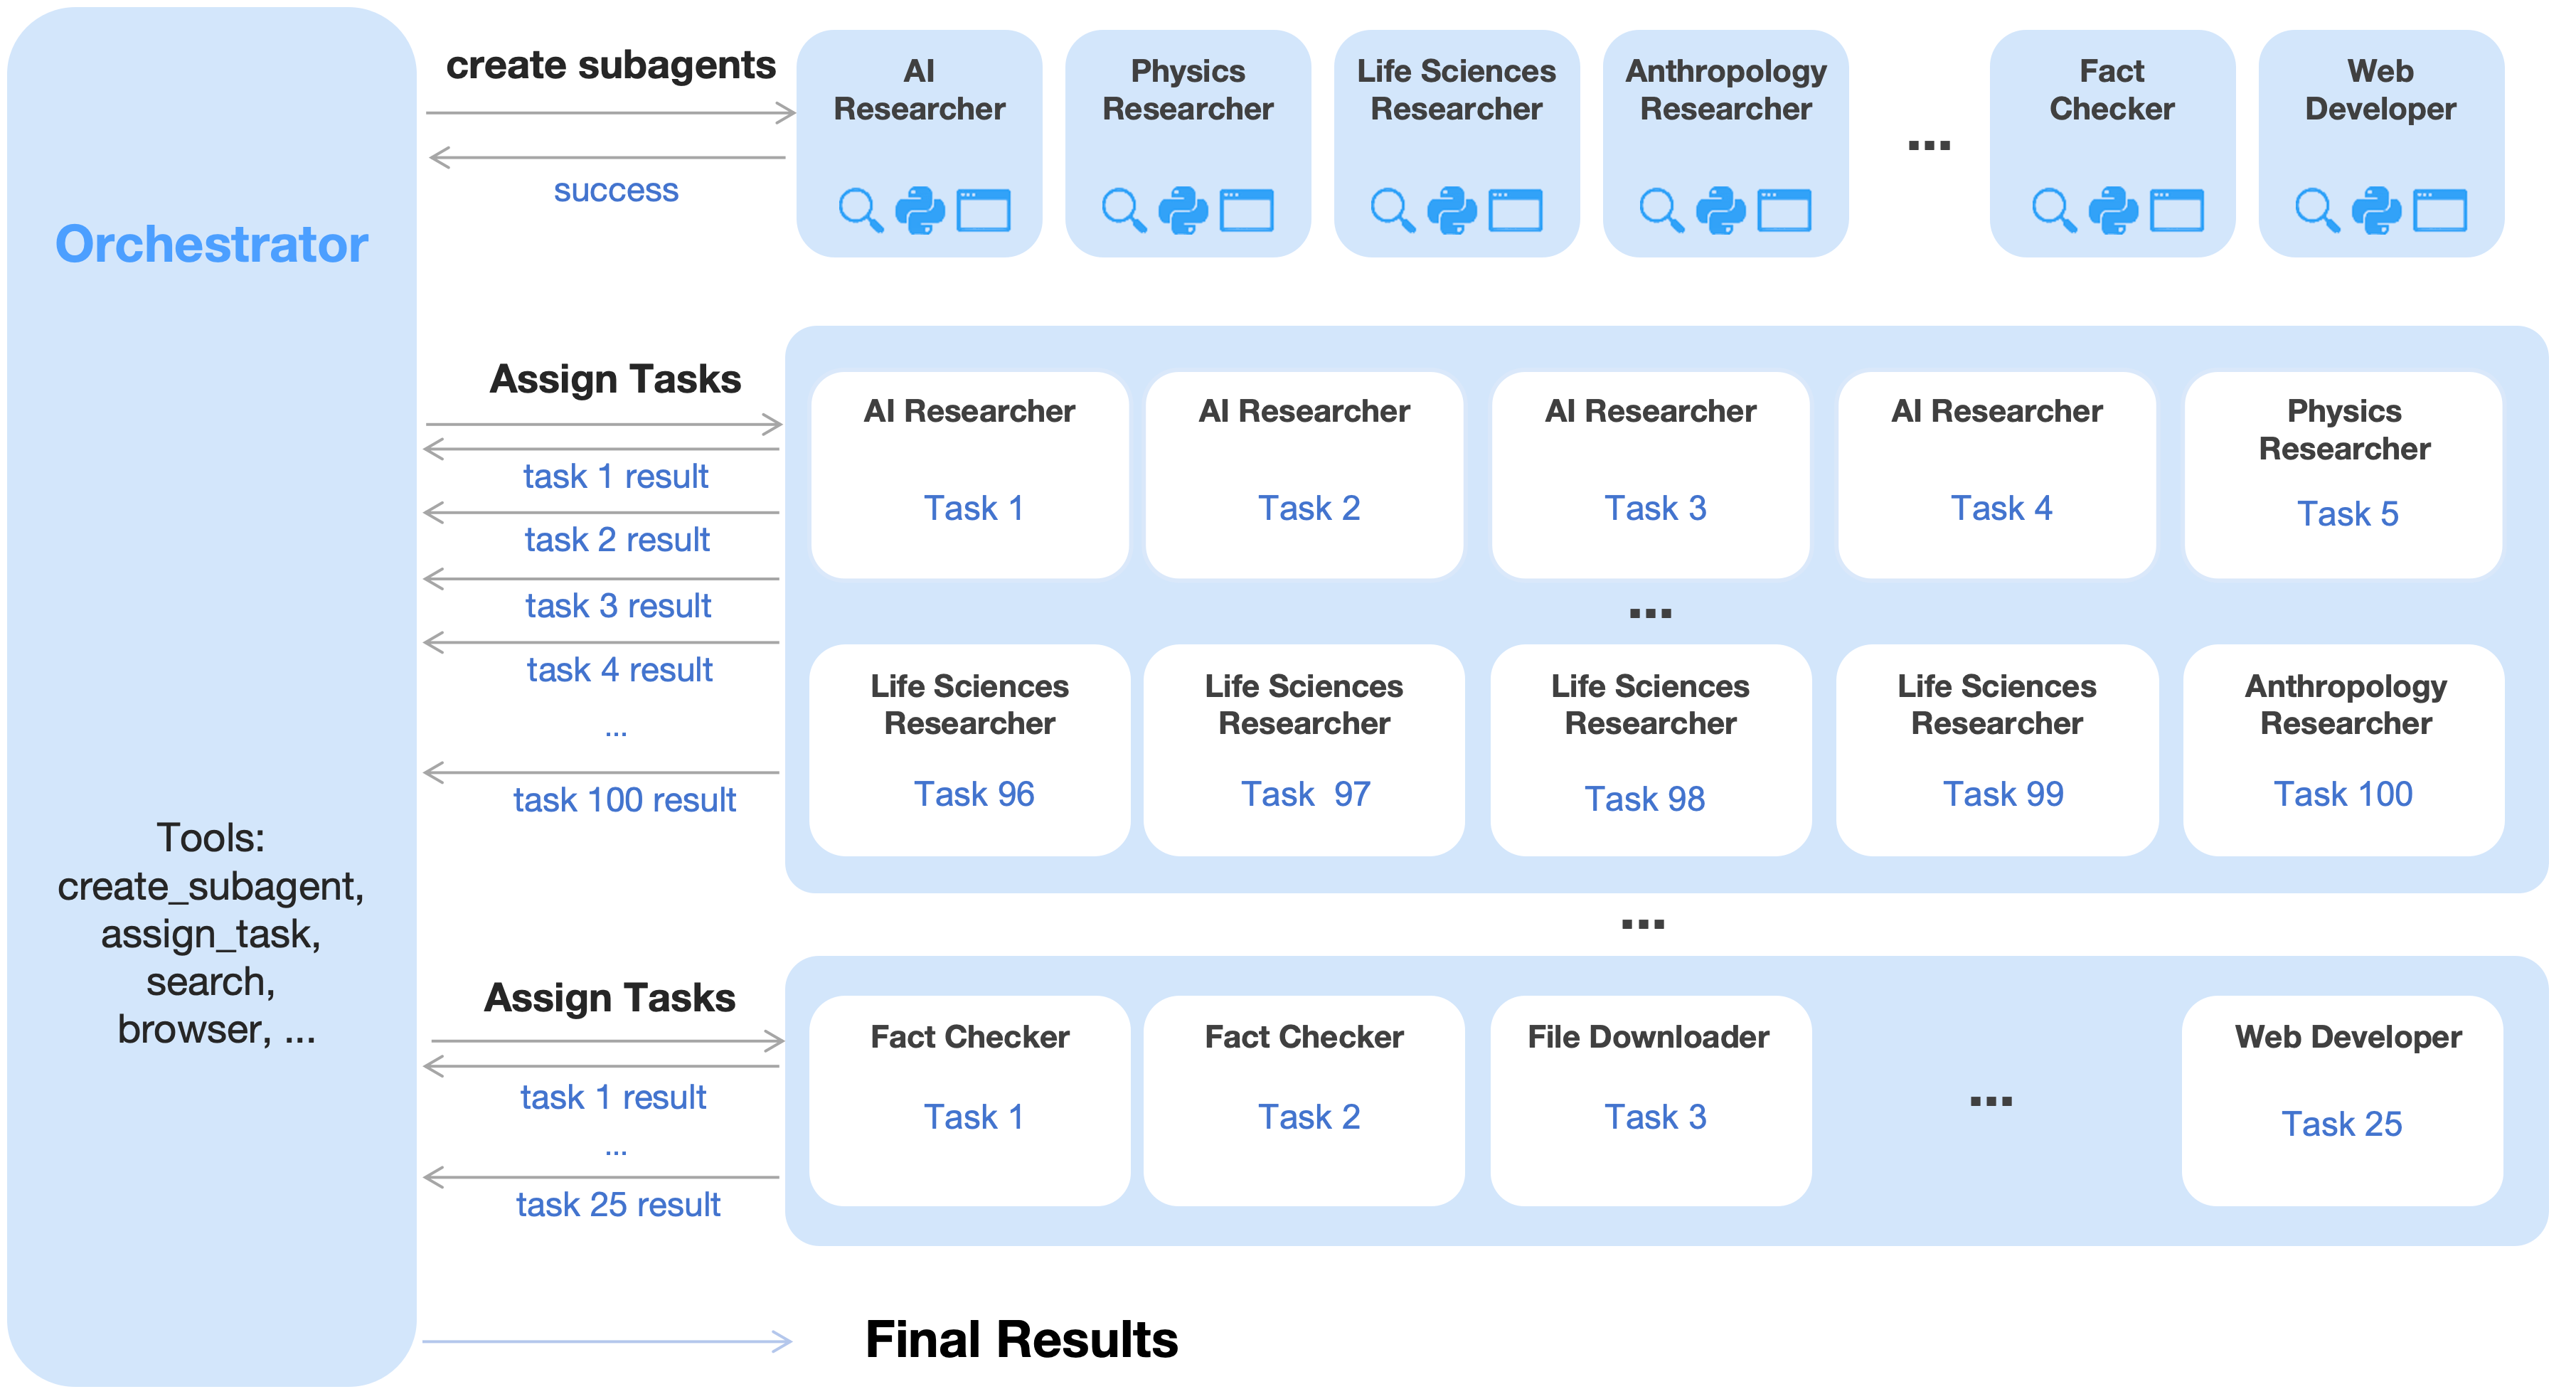
\includegraphics[width=0.9\linewidth]{figures/multi-agent-rl-system.png}
    \caption{An agent swarm has a trainable orchestrator that dynamically creates specialized frozen subagents and decomposes complex tasks into parallelizable subtasks for efficient distributed execution.}
    \label{fig:parl-orchestration}
\end{figure}
\paragraph{Architecture and Learning Setup} 

The PARL framework adopts a decoupled architecture comprising a trainable orchestrator and frozen subagents instantiated from fixed intermediate policy checkpoints. This design deliberately avoids end-to-end co-optimization to circumvent two fundamental challenges: credit assignment ambiguity and training instability. 
In this multi-agent setting, outcome-based rewards are inherently sparse and noisy; a correct final answer does not guarantee flawless subagent execution, just as a failure does not imply universal subagent error. 
By freezing the subagents and treating their outputs as environmental observations rather than differentiable decision points, we disentangle high-level coordination logic from low-level execution proficiency, 
 leading to more robust convergence.
To improve efficiency, we first train the orchestrator using small-size subagents before transitioning to larger models.
Our RL framework also supports dynamically adjusting the inference instance ratios between subagents and the orchestrator, thereby maximizing the resource usage across the cluster.


\paragraph{PARL Reward}
Training a reliable parallel orchestrator is challenging due to the delayed, sparse, and non-stationary feedback inherent in independent subagent execution. To address this, we define the PARL reward as:
\begin{align*}
r_{\mathrm{PARL}}(x, y) = \lambda_1 \cdot \mspace{-26mu} \underbrace{r_{\text{parallel}}}_{\text{instantiation reward}} \mspace{-9mu} + \mspace{18mu}\lambda_2 \cdot \mspace{-32mu}\underbrace{r_{\text{finish}}}_{\text{sub-agent finish rate}} + 
\underbrace{r_{\text{perf}}(x, y)}_{\text{task-level outcome}}
\, .
\end{align*}

The performance reward $r_{\text{perf}}$ evaluates the overall success and quality of the solution $y$ for a given task $x$. This is augmented by two auxiliary rewards, each addressing a distinct challenge in learning parallel orchestration. The reward $r_{\text{parallel}}$ is introduced to mitigate \emph{serial collapse}—a local optimum where the orchestrator defaults to single-agent execution. By incentivizing subagent instantiation, this term encourages the exploration of concurrent scheduling spaces. The $r_{\text{finish}}$ reward focuses on the successful completion of assigned subtasks. It is used to prevent \emph{spurious parallelism}, a reward-hacking behavior in which the orchestrator increases parallel metrics dramatically by spawning many subagents without meaningful task decomposition. By rewarding completed subtasks, $r_{\text{finish}}$ enforces feasibility and guides the policy toward valid and effective decompositions.

To ensure the final policy optimizes for the primary objective, the hyperparameters $\lambda_1$ and $\lambda_2$ are annealed to zero over the course of training.




\paragraph{Critical Steps as Resource Constraint} 
To measure computational time cost in a parallel-agent setting, we define \emph{critical steps} by analogy to the \emph{critical path} in a computation graph. 
We model an episode as a sequence of execution stages indexed by $t = 1, \dots, T$. 
In each stage, the main agent executes an action, which corresponds to either direct tool invocation or the instantiation of a group of subagents running in parallel. Let $S_{\mathrm{main}}^{(t)}$ denote the number of steps taken by the main agent in stage $t$ (typically $S_{\mathrm{main}}^{(t)} = 1$), and  $S_{\mathrm{sub},i}^{(t)}$ denote the number of steps taken by the $i$-th subagent in that parallel group. 
The duration of stage $t$ is governed by the longest-running subagent within that cohort. Consequently, the total critical steps for an episode are defined as 
\begin{align*}
\text{CriticalSteps}
= \sum_{t=1}^{T} \left( S_{\mathrm{main}}^{(t)} + \max_i S_{\mathrm{sub}, i}^{(t)} \right).
\end{align*}
By constraining training and evaluation using critical steps rather than total steps, the framework explicitly incentivizes effective parallelization. Excessive subtask creation that does not reduce the maximum execution time of parallel groups yields little benefit under this metric, while well-balanced task decomposition that shortens the longest parallel branch directly reduces critical steps. As a result, the orchestrator is encouraged to allocate work across subagents in a way that minimizes end-to-end latency, rather than merely maximizing concurrency or total work performed.


\paragraph{Prompt Construction for Parallel-agent Capability Induction}
To incentivize the orchestrator to leverage the advantages of parallelization, we construct a suite of synthetic prompts designed to stress the limits of sequential agentic execution. 
These prompts emphasize either \emph{wide search}, requiring simultaneous exploration of many independent information sources, or \emph{deep search}, requiring multiple reasoning branches with delayed aggregation. We additionally include tasks inspired by real-world workloads, such as long-context document analysis and large-scale file downloading. 
When executed sequentially, these tasks are difficult to complete within fixed reasoning-step and tool-call budgets. By construction, they encourage the orchestrator to allocate subtasks in parallel, enabling completion within fewer critical steps than would be feasible for a single sequential agent. Importantly, the prompts do not explicitly instruct the model to parallelize. Instead, they shape the task distribution such that parallel decomposition and scheduling strategies are naturally favored.



\begin{figure}[t]
    \centering
    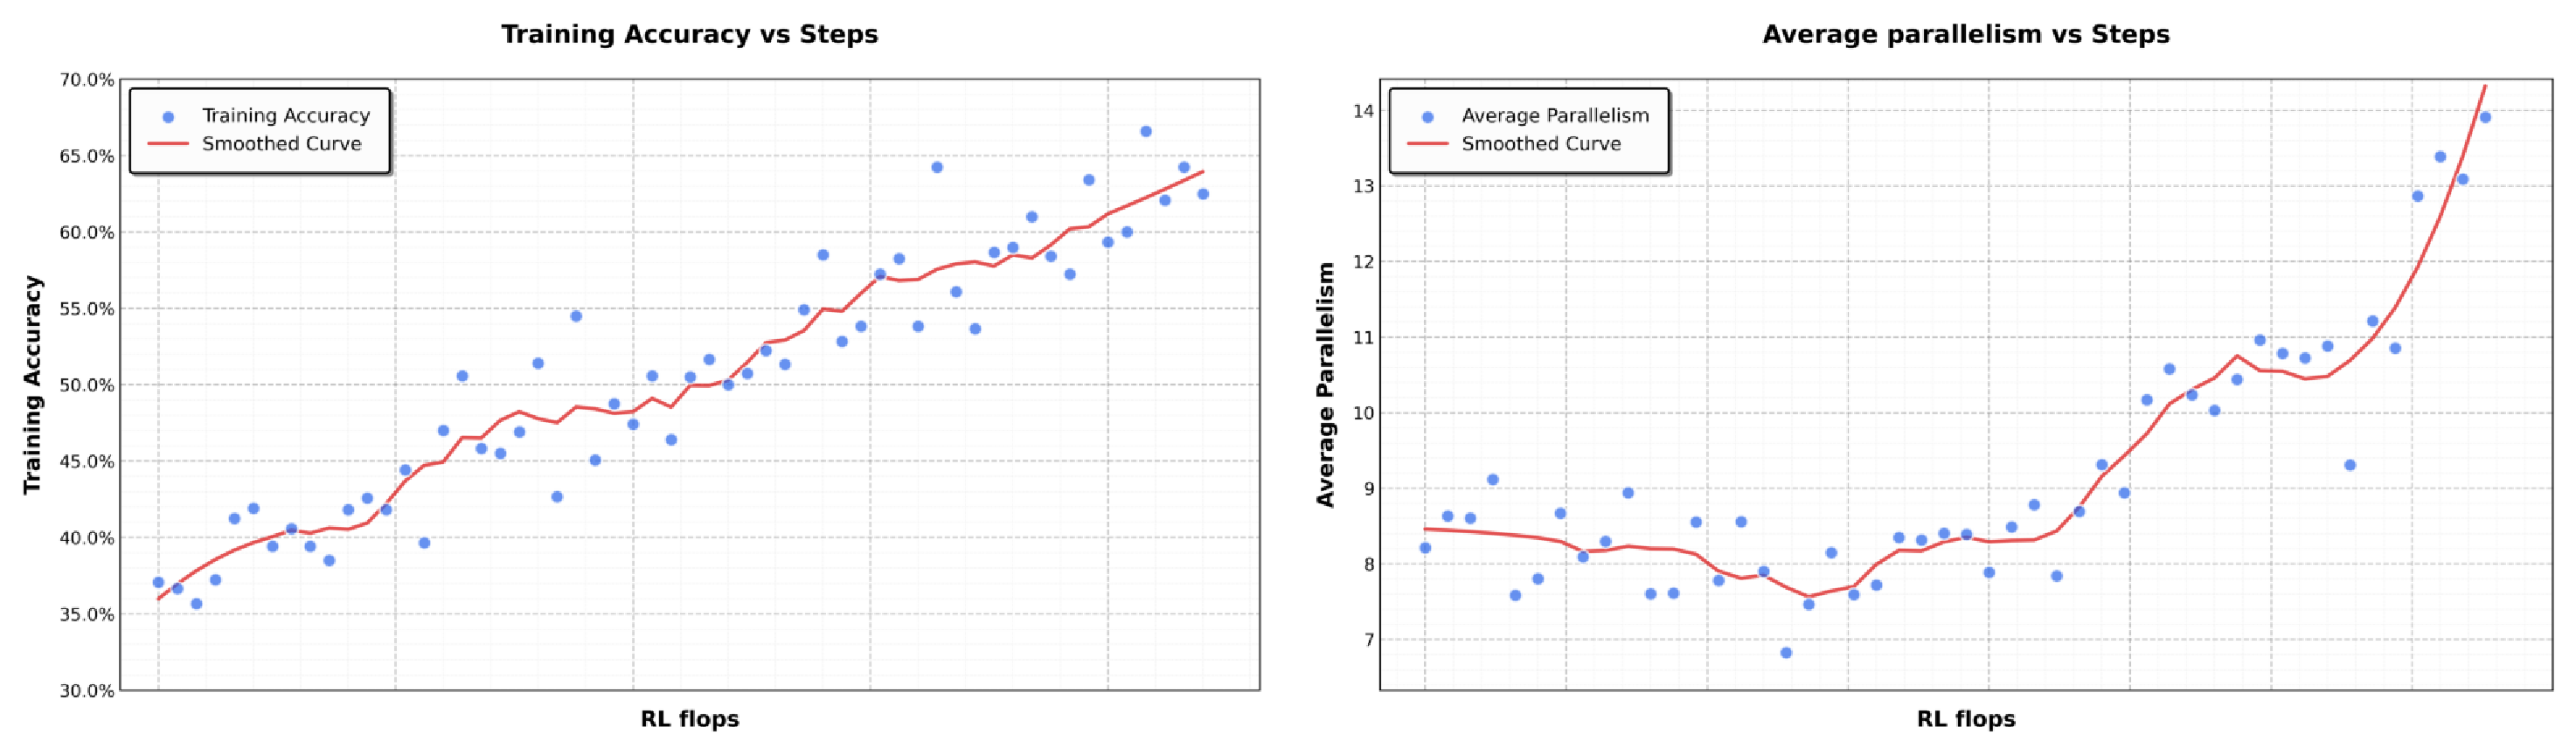
\includegraphics[width=\linewidth]{figures/pa-rl-progress.pdf}
    \caption{In our parallel-agent reinforcement learning environment, the training accuracy increases smoothly as training progresses. At the same time, the level of parallelism during training also gradually increases.}
    \label{fig:parl-learning}
\end{figure}
